\section{Results}

\begin{figure}[t]
	\centering
	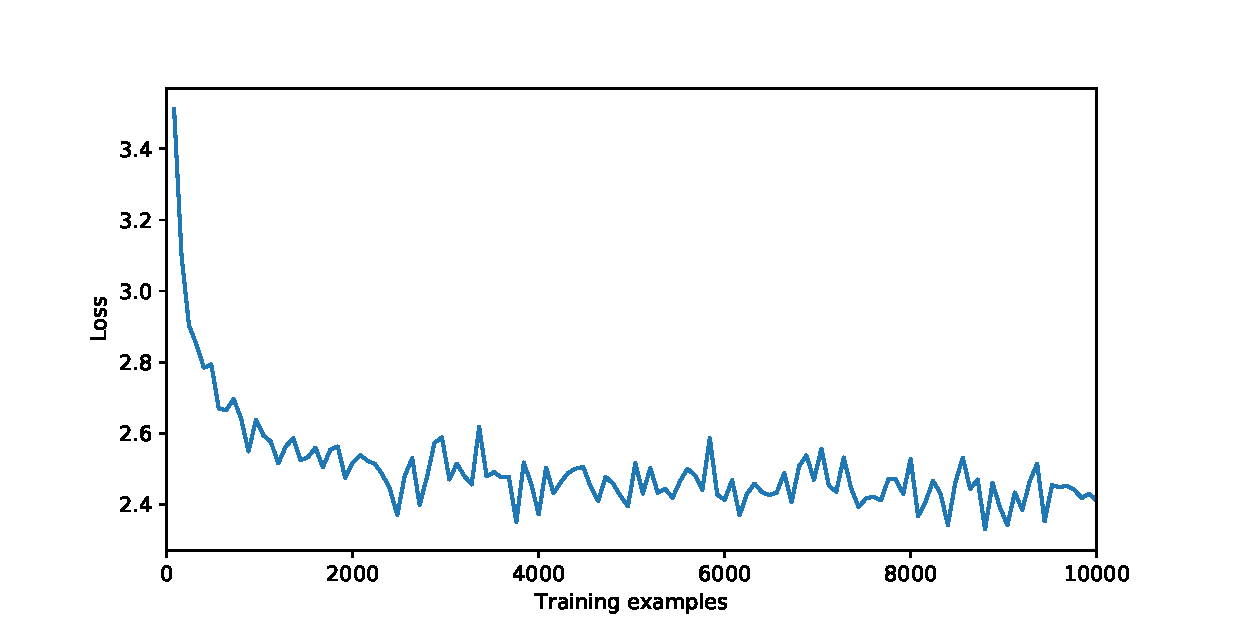
\includegraphics[width=0.8\textwidth]{figures/learning_curve.eps}
	\caption{The learning curve of training on 10,000 domain names.}
	\label{fig:learning_curve}
\end{figure}

\subsection{Training the network}
In order to train the network, the training set $T$ of 10,000 phishing domains was used. 
The domains were extracted from a set of phishing URLs\footnote{https://ecrimex.net/}, from which a set of the most popular domain names\footnote{https://www.alexa.com/topsites} was subtracted (e.g. {\tt docs.google.com}).
This subtraction of popular domains was done based on the assumption that popular domain names are not solely registered for phishing purposes, but are rather benign domain being abused for phishing purposes.

All domains were tokenized, transforming them from a string of characters to a one dimensional tensor of integers, where each integer represent a single character. 
The translation between characters and integers was stored in the alphabet of the model.
Before tokenizing, a start symbol {\tt <s>} and a end symbol {\tt </s>} were added to the domain in the start and end respectively. 
The start symbol was needed in order to eventually generate domain names without the need of providing a start symbol manually.
The end symbol was introduced for a similar reason, namely to the network to predict the end of a domain name.

For each domain $d$ in the training set, the model was trained as follows:
\begin{enumerate}
\item Initialize the hidden vector to zeroes.
\item For all characters $c_i$ in $d$ (except the last end symbol {\tt </s>}), take its subsequent character $c_{i+1}$ as the training target.
For instance, in the domain {\tt example.org}, the target for the first {\tt e} would be {\tt x}, and the target for {\tt g} would be {\tt </s>}.
\item Predict the output for $c_i$ and compute the loss between the output and the target $c_{i+1}$.
\item Back propagate the (clipped) total loss for domain $d$ through the network.
\end{enumerate}

Figure \ref{fig:learning_curve} shows the learning curve of the training phase of the network. 
The loss seems to converge to a value of around 2.5 after only 2000 domain names.

\subsection{Generating domains}
In order to start generating a new phishing domain name, the one-hot encoding of the start symbol {\tt <s>} and zero-initialized hidden vector is provided as input to the network.
Then, the network generates a logarithmic probability distribution for the next character based on the inputs.
From this probability distribution, a character is sampled and its one-hot encoding (in addition to last step's hidden output) is used as the input for the next step.
The generation algorithm runs until the network generates a {\tt </s>} symbol, or when the domain reaches a length of 255 characters (i.e. the maximum size of a domain name).
When sampling from the network, the dropout node is disabled, since sampling from the output probability distribution already introduces a stochastic element to the generation of domains.
For the discussion section, we generated the set $G$ of 10,000 domain names, the same size as the training set $T$.
The following shows a sample of generated domains:
\begin{verbatim}
14boerp.rom
comovecteboom.bozid.rom.com.d3
jkentr.in
m.pafreekakelesurtinvig.ooforeta.com
brefhatppaie.le-ipl-veri.ybaolutn.refymid.hogkid.s34-bsh.com
iocinsaide.po
www.chbong.hagel
sifienstle.hothunadragqwww.t-inlouig-ivglokh.cct.in
actaunl.gez
ppcus.iom
\end{verbatim}

